\documentclass{bioinfo}
%\usepackage{amsmath}
%\usepackage{enumerate}
\usepackage{graphicx}
%\usepackage[sorting=none]{biblatex}

%\author{Rusell~Y.~Neches, Elizabeth~.G.~Wilbanks, Philip~M.~ } 
%\title{Analyzing ChIP-seq data with Pique}

%\bibliography{writeup}

\copyrightyear{2012}
\pubyear{2012}

% This writeup is intended to be submitted to Bioinformatics as an
% Applicaiton Note under either the Gene Expression or Sequence
% Analysis. These are the instructions to authors :
%
% Application Notes (up to 2 pages; this is approx. 1300 words or 1000
% words plus one figure) : Applications Notes are short descriptions
% of novel software or new algorithm implementations, databases and
% network services (web servers, and interfaces). Software or data
% must be freely available to non-commercial users. Availability and
% Implementation must be clearly stated in the article. Authors must
% also ensure that the software is available for a full TWO YEARS
% following publication. Web services must not require mandatory
% registration by the user. Additional Supplementary data can be
% published online-only by the journal. This supplementary material
% should be referred to in the abstract of the Application Note. If
% describing software, the software should run under nearly all
% conditions on a wide range of machines. Web servers should not be
% browser specific. Application Notes must not describe trivial
% utilities, nor involve significant investment of time for the user
% to install.
%
% Software : If the manuscript describes new software tools or the
% implementation of novel algorithms the software must be freely
% available to non-commercial users at the time of submission, and
% appropriate test data should be made available. Availability must be
% clearly stated in the article. Authors must also ensure that the
% software and test data is available for a full TWO YEARS following
% publication. The editors of Bioinformatics encourage authors to make
% their source code available and, if possible, to provide access
% through an open source license (see www.opensource.org for
% examples). Authors should make every effort to use URLs that will
% remain stable. At the minimum, authors must provide one of:
% webserver, source code or binary.
%
% http://www.oxfordjournals.org/our_journals/bioinformatics/

\begin{document}
\firstpage{1}

\title[In a fit of pique]{Analyzing microbial ChIP-Seq data with
  Pique} \author[Neches
\textit{et~al}]{Russell~Y.~Neches\,$^{1,3}$\footnote{to whom
    correspondence should be addressed},
  Elizabeth~G.~Wilbanks\,$^{1,3}$, Phillip~M.~Seitzer,$^{2,3}$ and
  Marc~T.~Facciotti\,$^{2,3}$
  \address{$^{1}$Microbiology Graduate Group, University of California, Davis.\\
    $^{2}$Department of Biomedical Engineering, University of
    California, Davis.\\$^{3}$Genome Center, University of California,
    Davis.}}

\history{Received on XXXXX; revised on XXXXX; accepted on XXXXX}

\editor{Associate Editor: XXXXXXX}

\maketitle

\newcommand{\imsize}{1.0\columnwidth}
%\newcommand{\threeup}{0.26\columnwidth}
%\newcommand{\cotwo}{$\text{CO}_{2}$}
%\newcommand{\htwo}{$\text{H}_2$}
%\newcommand{\otwo}{$\text{O}_2$}
%\newcommand{\water}{$\text{H}_2\text{O}$}
%\newcommand{\htwos}{$\text{H}_2\text{S}$}

\begin{abstract}
\section{Motivation:}

\noindent While numerous effective peak finders have been developed
for eukaryotic systems, we have found that the approaches used can be
suprisingly error prone when run on high-coverage bacterial and
archaeal ChIP-Seq datasets.

% Why not? Examples, evidence, hypothesis. 

\section{Results:}

\noindent We have developed Pique, a conceptually simple, easy to use
ChIP-Seq peak finding application for bacterial and archaeal ChIP-Seq
experiments. The software is cross-platform and Open Source, and based
on only Open Source dependencies. Output is provided in standardized
file formats, and may be easily imported by the Gaggle Genome Browser
for manual curation and data exploration, or into statistical and
graphics software such as R for further analysis.

\section{Availability:} 

\noindent The software is available under the BSD-3 license at

\href{http://github.com/ryneches/pique}{http://github.com/ryneches/pique}.

\noindent A tutorial and test data are included with the documentation.

\section{Contact:} \href{ryneches@ucdavis.edu}{ryneches@ucdavis.edu}

\end{abstract}

\section{Introduction}

\noindent Next generation sequencing coupled with chromatin
immuno\-pre\-cipi\-tation (ChIP-Seq) is revolutionizing our ability to
genomically map protein-DNA interaction. The growing popularity of
ChIP-Seq has spurred the development of over thirty peak picking
algorithms (an extensive survey of these packages was conducted by
Wilbanks {\em et al.} \cite{wilbanks}). The relative performance of
representative peak detection algorithms on eukaryotic data, and
methods to assess performance have been recently reviewed by several
authors \cite{Pepke, Laajala_review, too_many_peak_callers,
  peakranger, peak_benchmark}.

While ChIP-Seq has been predominantly used to interrogate protein-DNA
interactions in eukaryotic systems, it is an especially powerful tool
for studying microbes. The small genomes and rapid growth rates, as
well as the extensive repertoire of experimental genetic tools
available for microbial systems permit ChIP-Seq to provide a
particularly clear picture of the sate of a cell's transcriptional
regulatory machinery.

However, only one ChIP-Seq analysis tool, CSDeconv \cite{CSDeconv},
has been explicitly developed for microbial data. This MATLAB package
successfully finds peaks in microbial ChIP-Seq data, but its
application is limited by its dependency on costly proprietary
software, slow performance, lack of support for manual
curation. Herein we describe Pique, a conceptually simple,
Python-based peak finding package that enables easy and rapid peak
finding in bacterial and archaeal ChIP-Seq datasets.

\section{Approach}

\noindent ChIP-Seq in bacteria and archaea yields coverage several
orders of magnitude larger than in eukaryotic systems, resulting in
continuous coverage rather than the sparse coverage typically present
in eukaryotic ChIP-Seq data.  This feature of microbial ChIP-Seq
experiments permits simpler, faster algorithms to be used. We have
based our algorithm on classic noise reduction techniques from signal
processing.

Pique is designed for use in systems that have genomic complexities
such as IS elements, gene dosage polymorphisms and accessory genomes
that cause coverage variations unrelated to ChIP, or in cases where
the organism under study is not identical to the reference genome. The
resulting enrichment ``pedestals'' and ``holes'' can be problematic
for detecting peaks and calculating enrichment levels. If the user
provides a map of these features, the software will automatically
perform a segmented analysis.

The wide variety of microbial systems, target proteins, protocols, and
experimental conditions calls for tailored statistical approaches to
ChIP-Seq. Rather than attempting to anticipate each of these (and
their combinations) with a very large number of statistical and
heuristic parameters, we have chosen to focus on the aspects of the
analysis that are common to all ChIP-Seq experiments; finding putative
peaks, estimating binding coordinates and binding affinities. The
determination of statistical significance is typically straightforward
for any particular experiment, but is quite difficult to robustly
generalize.

Pique allows users to create high-quality peak lists in two ways.
First, for each peak reported we report metrics that can be used to
ascertain which peaks are statistically significant (usually, this
involves little more than sorting the table and choosing a
cutoff). Second, we provide integrated support for curation using the
Gaggle Genome Browser. This permits interactive curation of the peak
list and analysis of the ChIP-Seq data in the context of other
Gaggle-enabled resources. Interactive curation of a microbial ChIP-Seq
data set can typically be completed in a few minutes.

\begin{methods}
\section{Methods}

\noindent Pique requires BAM files as input\cite{sam_format}.
Therefore, prior to using Pique, reads should first be quality
filtered, quality trimmed, and aligned to a reference genome (ideally,
all contigs of the reference genome should be used as the mapping
target).

By default, Pique treats each contig as a single analysis region, but
the user may designate regions within a contig for separate analysis.
This may be useful when coverage levels are systematically altered
over large regions.  Pique supports three features types; analysis
regions, masking regions, and normalization regions. Masking regions
are simply masked out of their respective analysis regions, and are
useful for removing coverage variation due to repetitive
DNA. Normalization regions selected within an analysis region are used
to compensate for total coverage discrepancies between the background
and ChIP alignments.

The user launches the analysis by providing alignment an file for the
ChIP data, an alignment file for the control data, and a coverage
feature map. The primary analysis proceeds as follows :

\begin{itemize}

\item The alignment files are digested into numeric coverage tracks,
  and the analysis regions are initialized in memory. Masking regions
  are applied.

%\item The coverage noise threshold is measured by comparing the total
%  coverage within the normalization regions between the ChIP data and
%  the control data. (Normalization regions must contain neither peaks
%  nor coverage level aberrations.)

% This no longer happens in the current version, as of August 18, 2011
%
%\item In each analysis region, the ``DC'' component is removed using
%  linear detrending. This removes effects due to coverage variation
%  features larger than about 100Kb.

\item High-$k$ noise is removed using a Wiener-Kolmogorov filter. The
  filter delay $\alpha$ is chosen to approximate to the expected
  footprint size of the targeted protein. The choice of filter implies
  the existence of two inputs; a ``true'' signal, and a noise
  source. Both are assumed to be stationary stochastic processes
  combined additively.

  % The Wiener-Kolmogorov filter was the first and simplest
  % statistical signal filter, first published by Norbert Wiener in
  % 1949, and independently derived in discrete-time form by Andrey
  % Kolmogorov in 1941.

\item A Blackman window of a diameter equal to the read length is
  convolved with the filtered coverage track to remove features
  smaller than one read. This reduces the effect of fragmentation
  position bias, and may be especially useful when transposon-based
  library construction is used.

\item The noise threshold in the ChIP coverage track is measured by
  comparing the coverage distribution in the ChIP track to the control
  track within user-annotated non-peak regions. Features that exceed
  the noise threshold are identified.

\item Because read orientations are constrained by the fragment size,
  binding events cause a offset enrichment between the forward and
  reverse strands. Pique exploits this by requiring that the stop
  coordinate of the forward strand enrichment envelope must fall
  between the coordinates of the reverse strand enrichment envelope,
  and that the start coordinate of the reverse strand enrichment
  envelope fall between the coordinates of the forward strand
  enrichment envelope. (We call this the overlap criterion.)

\end{itemize}

\begin{figure}[!tfbd data - reasonable spot showing curation]%figure2
  \begin{center}
    {\resizebox{\imsize}{!}{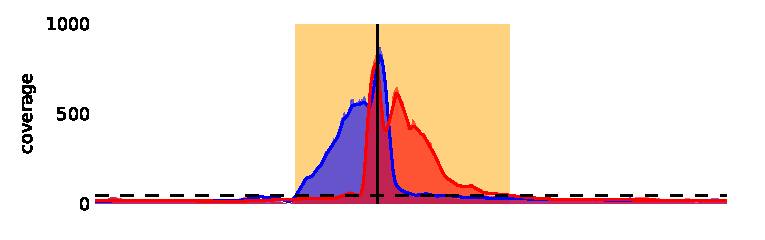
\includegraphics{peak_example.pdf}}}
    {\resizebox{\imsize}{!}{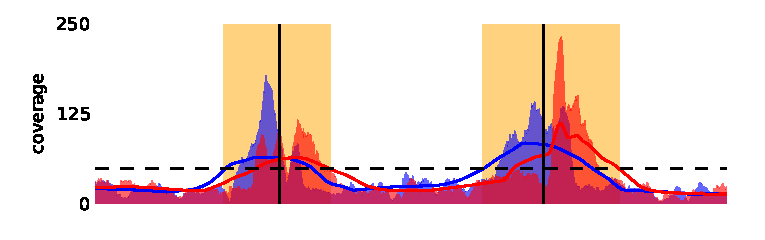
\includegraphics{peak_example_2.pdf}}}
  \end{center}
  \caption{Peaks found in the included sample dataset, derived from
    ChIP-seq of tfbD in {\em Halobacterium salinarum} sp. NRC1. Blue
    and red shading indicate coverage of reads aligned from the
    ChIP-derived data to the forward and reverse strands,
    respectively. Blue and red lines represent the filtered coverage
    levels for the forward and reverse strands, respectively. The
    dashed line is the detected noise threshold for the
    region. Detected peaks are indicated in orange
    boxes.}\label{fig:02}
\end{figure}

\noindent For each putative peak, Pique calculates the enrichment
ratio of the ChIP alignment to the control alignment, the binding
coordinate, and the enrichment normalization factor for that analysis
region. 

\end{methods}

% \begin{figure}[!tfbd peak - a nice one]%figure1
%   % \centerline{\includegraphics{example_data.png}
%   \begin{center}
%     {\resizebox{\imsize}{!}{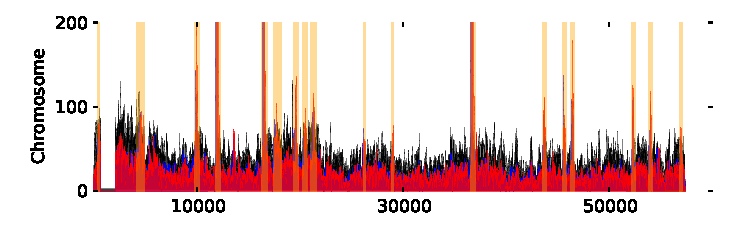
\includegraphics{chr_example.pdf}}}
%     %{\resizebox{\imsize}{!}{\includegraphics{../PNRC200_0:21851.pdf}}}
%     %{\resizebox{\imsize}{!}{\includegraphics{../PNRC200_47121:88549.pdf}}}
%   \end{center}
%   \caption{Peaks found in the chromosome of the included sample
%     dataset, derived from ChIP-seq of tfbD in {\em Halobacterium
%       salinarum} sp. NRC1. Blue and red indicate coverage of reads
%     aligned from the ChIP-derived data to the forward and reverse
%     strands of the genome, respectively. Black indicates coverage
%     aligned from the whole cell extract data. Orange indicates a
%     detected peak. The maximum coverage in this data is 3204, but is
%     shown here truncated at 200.}\label{fig:01}
% \end{figure}

\section{Results}

Performance of Pique was benchmarked against CSDeconv two ChIP-Seq
experiments. The first experiment targeted TfbD (transcription
initiation factor IIB 4) DNA-binding events in late stationary phase
of {\em Halobacterium salinarum} sp. NRC1 described in Wilbanks {\em
  et al.} \cite{wilbanks}. Peak lists for both Pique and CSdeconv were
compared with experimentally verified transcription start sites
collected by Koide {\em et al} \cite{halo_promoters} and scanned for
the presence of putative binding motifs using MAST\cite{MAST}. An {\em
  ab initio} search for putative binding motifs in each peak list was
conducted, and the recovered motifs compared using STAMP \cite{STAMP}.

The second experiment targeted the DosR (dormancy survival regulator)
DNA-binding events after two hours exposure to oxygen after growth to
early log phase of {\em Mycobacterium tuberculosis} described in Lun
{\em et al.}  \cite{CSDeconv}. To the best of our knowledge,
transcription start sites have not been systematically verified
experimentally in this organism, and so putative transcription start
sites were identified using the putative binding motif found
constructed by Gerasimova {\em et al.} \cite{DosR_motif} using
MAST. An {\em ab initio} search for putative binding motifs was
conducted, and the recovered motifs compared using STAMP.  

\subsection{TfbD in {\em Halobacterium salinarum} sp. NRC1}

The putative TfbD binding motif for this organism is analogous to
[???] a similar archaeon's TFB protein in photocrosslinking study
\cite{tfb_promoter}, and is thought to consist of a TFB recognition
element (BRE), a TATA box, a proximal promoter element (PPE) and a
transcription start site (TSS). This putative promoter motif was
scanned against each peak region using MAST \cite{MAST} with an
$e$-value cutoff of 100 and the default motif $p$-value cutoff of
$10^{-4}$. Peaks found by each software package were also for presence
of experimentally determined transcript start sites (TSS)
\cite{halo_promoters} (Table \ref{table1}).

\begin{table}
  \begin{center}
    \begin{tabular}{l r r r r}
      Found by & Peaks & TSS & Motif & TSS \& Motif \\
      \hline
      Pique or CSDeconv & 610 & 332 & 197 & 69 \\
      Pique             & 417 & 225 & 128 & 50 \\
      CSDeconv          & 449 & 213 & 138 & 50 \\
      Pique \& CSDeconv & 257 & 106 & 69  & 31 \\
      Pique only        & 160 & 119 & 59  & 19 \\
      CSDeconv only     & 192 & 107 & 69  & 19 \\
    \end{tabular}
  \end{center}
  \caption{Putative binding motifs and transcript start sites detected 
    in peaks recovered by Pique and CSDeconv.}\label{table1}
\end{table}

Enrichment ratios (the ratio of the integrated coverage to the
background) for each peak were calculated, and peaks from each
software package for each category were then placed in rank order
(Fig. \ref{ranked_peaks}). It was found that Pique recovered more
peaks than CSDeconv, and more peaks with experimentally verified
transcript start sites. It was found that Pique and CSDeconv recovered
peaks containing the full putative binding motif (BRE-TATA-PPE-TSS) at
the same rate.

\begin{figure}
  \begin{center}
    {\resizebox{\imsize}{!}{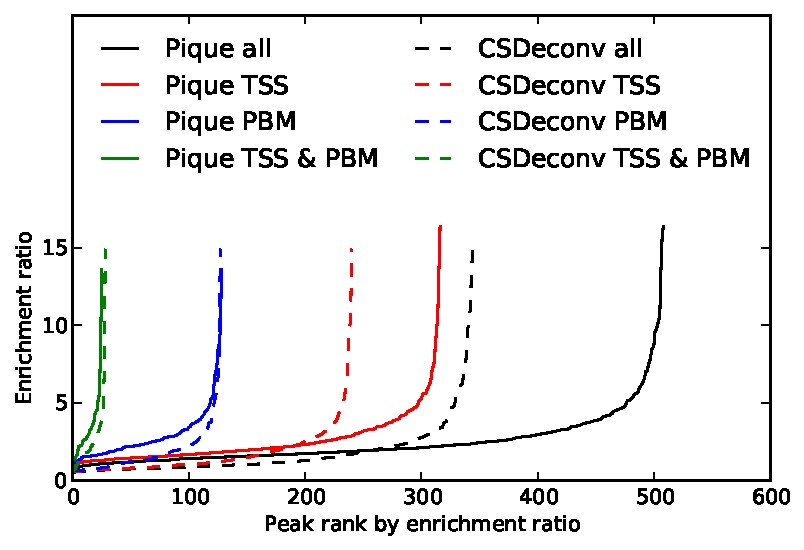
\includegraphics{pique_csd_ranks.pdf}}}
  \end{center}
  \caption{Performance of Pique and CSDeconv on a ChIP-seq experiment
    ({\em Halobacterium salinarum} sp. NRC1 transcription initiation
    factor TFB tfbD in late stationary phase) was studied by comparing
    lists of peaks. Peak lists are shown here ranked by enrichment
    ratio. Pique recovers more peaks than CSDeconv, and more of these
    peak regions contain an experimentally determined transcription
    start site (TSS). Both software packages recovered the same number
    of peaks containing the predicted binding motif (PBM). Both
    software packages recovered the same number of peaks in which a
    transcript start site was found less than 50bp downstream from a
    binding motif. TSS coordinates were experimentally verified (Koide
    {\em et al.}) \cite{halo_promoters} and motifs were predicted
    using Motif Catcher (Seitzer {\em et al.}, publication
    pending).}\label{ranked_peaks}
\end{figure}

In order to ascertain the quality of the predicted peak regions
uniquely predicted by each software package, an {\em ab initio} search
for the putative binding motif was conducted for each list of peaks. 

Sequence entries were created by extracting 100-bp stretches of
sequence centered at each respective called peak center.  Each
sequence data set was subjected to an iterative MC MAST/MEME
MotifCatcher search [3] with 100 seeds. This search was conducted for
five groups of sequences corresponding to all peak regions found by
Pique, regions found exclusively by Pique, all peak regions found by
CSDeconv, regions found by CSDeconv exclusively, and peak regions
found by both software packages. Motifs could be discovered on the
forward and reverse strand, and could be anywhere from 20 to 40
nucleotides in length (Supplementary Figure 2). A putative binding
motif was discovered in all five sets of peaks.

The pairwise distances between motifs was computed by the average log
likelihood ratio (ALLR), and clustered using UPGMA (program
defaults). All motifs that were significantly similar to the putative
canonical TFB motif were clustered, and for cases where more than two
significant motif matches were discovered in a given data set, motifs
were clustered and familial profiles were computed. Membership
clustering thresholds were tried from 0 to 1.0 in increments of 0.10,
and the familial profile motif with the lowest $e$-value was taken
from each dataset as its ``representative'' motif profile.  For cases
where two or fewer significant motif matches were determined, the
motif match with the lower $e$-value was taken as the representative
motif profile of its respective data set. Representative motifs were
compared using STAMP \cite{STAMP} with the ALLR motif comparison
measure and UPGMA clustering (Fig. \ref{motif-tree}).

\begin{figure}
  \begin{center}
    {\resizebox{\imsize}{!}{\includegraphics{motif-tree.pdf}}}
  \end{center}
  \caption{Motifs recovered by Pique and CSDeconv are qualitatively
    different.}\label{motif-tree}
\end{figure}

It was found that the motifs computed from the list of peak regions
recovered by Pique and CSDeconv clustered closely with the canonical
binding motif, as did motifs computed from the list of peak regions in
common to both software packages. However, motifs computed from the
list of peak regions recovered {\em exclusively} by Pique clustered
with the canonical motif, but the motifs computed from the list of
peak regions recovered {\em exclusively} by CSDeconv did not
(Fig. \ref{motif-tree}). Furthermore, the $e$-value of the best motif
computed from the CSDeconv-unique peak regions is the lowest among the
five, suggesting that a higher proportion of false positives may be
among this list.

\begin{table}
  \begin{center}
    \begin{tabular}{ l l }
      Peak list & Motif $e$-value \\
      \hline
      CSDeconv all      & $3.3 \times 10^{-144}$ \\
      CSDeconv only     & $5.2 \times 10^{-35}$ \\
      Pique \& CSDeconv & $6.9 \times 10^{-77}$ \\
      Pique all         & $4.6 \times 10^{-130}$ \\
      Pique only        & $4.9 \times 10^{-82}$ \\
    \end{tabular}
  \end{center}
  \caption{Statistical support for motifs computed from lists of peaks 
    found by Pique and CSDeconv.}
\end{table}

\subsection{DosR in {\em Mycobacterium tuberculosis}}


\section{Discussion}

Pique does not attempt to filter peaks that are statistically
insignificant. We have found that this part of the analysis is usually
specific to the data and to the experiment, and can be highly
idiosyncratic. Pique is designed to achieve a low false-negative
rate. This allows Pique to work without modification on many different
kinds of experiments, but at the cost of some post-filtering. Pique
provides the user with output that can be used to support a variety of
such statistical tests.

Some recommended filtering might include eliminating peaks that are
significantly narrower than the size range of the sequencing library,
peaks with a normalized enrichment ratio below unity, or peaks that
have predicted binding sites that are very skewed from the center of
the enriched region. Depending on how many peaks are recovered, the
user may wish to try one or all of these, perhaps with
clustering. However, if a ``perfect'' peak list is required, we have
found that heuristic filtering is inadequate regardless of the
software used. To facilitate manual curation, Pique outputs a track
file of the coverage, a quantitative positional data of the estimated
binding sites, and a bookmark file annotating the peaks. These files
are simple to process by a variety of tools, and can be loaded
directly into the Gaggle Genome Browser. False positives are easy to
recognize visually, and can be easily deleted.\footnote{See
  supplementary figure.}







\section{Conclusion}

We conclude that Pique provides a rapid, open source platform for the
sensitive detection of transcription factor binding sites in bacterial
and archaeal ChIP-seq experiments. We leverage standard signal
processing algorithms to rapidly identify binding sites. Downstream
analysis is supported via integration with statistical and graphics
software such as R, and curation via integration with the
user-friendly Gaggle Genome Browser and the suite of Gaggle tools.

We note that Pique should also work well with eukaryotic datasets
provided they are gathered with greater coverage than has been
previously reported.

\section*{Acknowledgement}
\paragraph{Funding\textcolon} 

This project was funded by UC Davis startup funds to M.T.F., NSF Graduate
Research Fellowship awarded to E.G.W. and DARPA award number
HR0011-05-1-0057 to R.Y.N.

\bibliographystyle{unsrt}
%\bibliographystyle{achemnat}
%\bibliographystyle{plainnat}
%\bibliographystyle{abbrv}
%\bibliographystyle{bioinformatics}

%\bibliographystyle{plain}

\bibliography{writeup}

\end{document}